\documentclass[hidelinks,11pt,final]{article}
\usepackage{bbm}
\usepackage[english]{babel}
\usepackage[utf8]{inputenc}
\usepackage{graphicx}
%\usepackage{lmodern}
\graphicspath{{../img/}} 
\usepackage[noend]{algorithm2e}
\usepackage[margin=1in]{geometry}
\usepackage{caption}
\usepackage{mathtools}
\usepackage{amsmath}
\usepackage{amsthm}
\usepackage{amssymb}
\usepackage{appendix}
%\usepackage{wasysym}
\usepackage{hyperref}
\usepackage[square,numbers]{natbib}

\newcommand{\envnumstyle}{section}
\newcounter{proofeqcounter}
\AtBeginEnvironment{proof}{\setcounter{proofeqcounter}{\value{equation}}
\setcounter{equation}{0}\renewcommand{\theequation}{\alph{equation}}}
\AtEndEnvironment{proof}{\setcounter{equation}{\value{proofeqcounter}}}

\theoremstyle{plain}
\newtheorem{theorem}{Theorem}[\envnumstyle]
\newtheorem{corollary}{Corollary}[theorem]
\newtheorem{definition}{Definition}[\envnumstyle]
\newtheorem{postulate}{Postulate}[\envnumstyle]
\newtheorem{conjecture}{Conjecture}[\envnumstyle]

\newtheorem{assumption}{Assumption}

\newcounter{examplecounter}

\newenvironment{example}
{
    \refstepcounter{examplecounter}%
    \par\vspace{\baselineskip}\noindent 
    \textbf{Example \theexamplecounter}%
    \begin{itshape}
    \quad
}
{
    \end{itshape}
    \par\vspace{\baselineskip}% 
    \noindent\ignorespacesafterend     
}

\newcounter{exampleeqcounter}
\AtBeginEnvironment{example}{\setcounter{exampleeqcounter}{\value{equation}}
\setcounter{equation}{0}\renewcommand{\theequation}{\alph{equation}}}
\AtEndEnvironment{example}{\setcounter{equation}{\value{exampleeqcounter}}}

\newtheorem*{remarkx}{Remark}
\newenvironment{remark}
  {\pushQED{\qed}\renewcommand{\qedsymbol}{$\triangle$}\remarkx}
  {\popQED\endremarkx}

\newtheorem*{notation}{Notation}


\SetKwFunction{sampler}{sample\_bit\_length}
\SetKwFunction{makehash}{make\_perfect\_hash}
\SetKwFunction{PerfHash}{perfect\_hash}

\RestyleAlgo{ruled}
\LinesNumbered
\newcommand{\COMMENT}[1]{}
\newcommand{\cat}{\mathbin{\#}}
\newcommand{\BL}{\mathrm{BL}}
\newcommand{\Fun}[2][]{\mathrm{#2}_{#1}}
\newcommand{\PH}{\mathrm{PH}}
\newcommand{\ph}{\mathrm{ph}}
\newcommand{\PS}[1]{\mathcal{P}(#1)}
\DeclareMathOperator*{\argmax}{arg\,max}
\newcommand{\MinHash}{\mathrm{min\_hash}}
\newcommand{\MaxHash}{\mathrm{max\_hash}}
\newcommand{\geodist}{\mathrm{Geometric}}
\newcommand{\Expect}[1]{\mathbb{E}\left[#1\right]}
\newcommand{\Break}{\textbf{break}}
\newcommand{\True}{\textbf{true}}
\newcommand{\False}{\textbf{false}}



\hypersetup{
    pdftitle={Cryptographic perfect hash functions: A theoretical analysis on space efficiency and entropy},                    % title
    pdfauthor={Alexander Towell},               % author
    pdfsubject={computer science},              % subject of the document
    pdfkeywords={
        perfect hash function,
        random oracle,
        space complexity,
        maximum entropy,
        cryptographic hash function},           % keywords
    colorlinks=false,                           % false: boxed links; true: colored links
    citecolor=green,                            % color of links to bibliography
    filecolor=magenta,                          % color of file links
    urlcolor=green                              % color of external links
}

\title
{
    Cryptographic perfect hash functions\\
    \large A theoretical analysis on space efficiency and algebraic composition
}

\author
{
    Alexander Towell\\
    \texttt{lex@metafunctor.com}
}
\date{}

\PassOptionsToPackage{unicode}{hyperref}
\PassOptionsToPackage{naturalnames}{hyperref}

\begin{document}
\maketitle
\begin{abstract}
We analyze a theoretical \emph{perfect hash function} that has three desirable properties: (1) it is a cryptographic hash function; (2) its \emph{in-place} encoding obtains the theoretical lower-bound for the expected space complexity; and (3) its \emph{in-place} encoding is a random bit string with maximum entropy.
\end{abstract}

\textbf{Keywords:} perfect hash function,
        random oracle, space complexity,
        maximum entropy, cryptographic hash function

\tableofcontents

%####################################################################################################
% prior art
%####################################################################################################

\section{Prior Art}
Perfect hash functions have been extensively studied in the literature. The seminal work of Fredman, Koml\'{o}s, and Szemer\'{e}di~\cite{fks} established that static dictionaries can be stored in linear space with $O(1)$ worst-case lookup time, laying the theoretical foundation for perfect hashing. Dietzfelbinger et al.~\cite{phf} extended these results to dynamic settings, establishing theoretical bounds for space-efficient hash tables with worst-case constant access time. Czech, Havas, and Majewski~\cite{pmf} introduced practical families of perfect hashing methods that became widely influential.

More recent practical algorithms have focused on minimal perfect hash functions (MPHFs), which achieve a load factor of exactly 1. Botelho, Pagh, and Ziviani~\cite{simple} presented simple and space-efficient constructions, while Belazzougui, Botelho, and Dietzfelbinger~\cite{chd,mphfsurvey} developed the Compress, Hash, and Displace (CHD) algorithm, which achieves excellent space-time tradeoffs for large datasets. Related techniques such as cuckoo hashing~\cite{cuckoo} provide alternative approaches to collision resolution with strong theoretical guarantees.

From an information-theoretic perspective, Shannon's foundational work~\cite{shannon} established the theoretical limits of data compression, which directly inform the space lower bounds for perfect hash functions. Cover and Thomas~\cite{coverandthomas} provide a comprehensive treatment of entropy and optimal coding, which underpin the analysis of encoding efficiency in this paper.

The random oracle model, introduced by Bellare and Rogaway~\cite{randomoracle}, provides a theoretical framework for analyzing cryptographic hash functions as ideal random functions. This model is central to our analysis, as it allows us to derive precise probability distributions for the search process in Algorithm~\ref{alg:ph}.

Our work differs from prior approaches by focusing on the theoretical properties of cryptographic perfect hash functions with maximum entropy encodings. While practical algorithms prioritize construction speed and space efficiency, we analyze the fundamental information-theoretic properties of perfect hash functions when the underlying hash function is modeled as a random oracle. This perspective reveals that the in-place encoding of such functions achieves the theoretical entropy bound, providing a rigorous foundation for understanding the space-optimality of perfect hash constructions.

%####################################################################################################
% perf hash fn
%####################################################################################################

\section{Perfect hash functions}
A \emph{set} is an unordered collection of distinct elements.
If we know the elements in a set, we may denote the set by these elements, e.g., $\{a,c,b\}$ denotes a set whose members are exactly $a$, $b$, and $c$.

A \emph{finite set} has a finite number of elements.
For example, $\{ 1, 3, 5 \}$ is a finite set with three elements.
When sets $\mathbbm{A}$ and $\mathbbm{B}$ are \emph{isomorphic}, denoted by $\mathbbm{A} 
\cong \mathbbm{B}$, they can be put into a one-to-one correspondence (bijection), e.g., $\{b,a,c\} \cong \{1,2,3\}$.
Since there exists at least one bijection between isomorphic sets, we can losslessly convert one to the other and thus, isomorphic sets are in some sense equivalent.

The cardinality of a finite set $\mathbbm{A}$ is the number of elements in the set, denoted by $|A|$, e.g., $|\{ 1, 3, 5\}| = 3$.
A \emph{countably infinite set} is isomorphic to the set of \emph{natural numbers} $N = \{1,2,3,4,5,\ldots\}$.

Given two elements $a$ and $b$, an ordered pair of $a$ then $b$ is denoted by $(a,b)$, where $(a,b) = (c,d)$ \emph{if and only if} $a = c$ and $b = d$.
Ordered pairs are non-commutative and non-associative, i.e., $(a,b) \neq (b,a)$ if $a \neq b$ and $(a,(b,c)) \neq (b,(a,c))$.

Related to the ordered pair is the Cartesian product.
\begin{definition}
The set $\mathbbm{X} \times \mathbbm{Y} = \left\{(x,y) : x \in 
\mathbbm{X} \land y \in \mathbbm{Y}\right\}$ is the Cartesian product of sets $\mathbbm{X}$ 
and $\mathbbm{Y}$.
\end{definition}
By the non-commutative and non-associative property of ordered pairs, the Cartesian product is non-commutative and non-associative.
However, they are isomorphic, i.e., $\mathbbm{X} \times \mathbbm{Y} \cong \mathbbm{Y} \times \mathbbm{X}$.

A \emph{tuple} is a generalization of order pairs which can consist of an arbitrary number of elements, e.g., $(x_1,x_2,\ldots,x_n)$.
\begin{definition}[$n$-fold Cartesian product]
The $n$-ary Cartesian product of sets $\mathbbm{X}[1],\ldots,\mathbbm{X}[n]$, is given by $\mathbbm{X}[1] \times \cdots \times \mathbbm{X}[n] = \left\{(x_1,\ldots,x_n) : x_1 \in \mathbbm{X}[1] \land \cdots \land x_n \in \mathbbm{X}[n]\right\}$.
\end{definition}
Note that $\mathbbm{X}[1] \times \mathbbm{X}[2] \times \mathbbm{X}[3] \cong \mathbbm{X}[1] \times \left(\mathbbm{X}[2] \times \mathbbm{X}[3]\right) \cong \left(\mathbbm{X}[1] \times \mathbbm{X}[2]\right) \times \mathbbm{X}[3]$, thus we may implicitly convert between them without ambiguity.

If each set in the $n$-ary Cartesian product is the same, the power notation may be used, e.g., $\mathbbm{X}^3 \equiv \mathbbm{X} \times \mathbbm{X} \times \mathbbm{X}$.
As special cases, the $0$-ary (nullary) Cartesian product is defined to be $\{ \emptyset \}$, and the $1$-ary (unary) Cartesian product is the identity, e.g., $\mathbbm{X}^1 = \mathbbm{X}$.



%\begin{example}
%Consider the number $100$ (base $10$). To determine the bit string $100'$, we perform the following steps:
%\begin{enumerate}
%    \item The length of $100'$ is $\lfloor \log_2 100 \rfloor = 6$.
%    \item Subtract $2^6 = 64$ from $100$ which results in $36$.
%    \item $36_{10}$ in binary is $100100_2$.
%    \item $100' = (1\,0\,0\,1\,0\,0)$.
%\end{enumerate}
%\end{example}

%A similar mapping may be defined for $\{0,1\}^m$ and $\{1,2,\ldots,2^m\}$ as given by
%\begin{equation}
%    b_m \mapsto \sum_{j=1}^{m} 2^{m - j + 1} b_j,
%\end{equation}
%where $b_m \in \{0,1\}^m$.
%   1   empty
%   2   0       
%   3   1
%   4   00
%   5   01
%   6   10
%   7   11
%   8   000
%   9   001
%   10  010
%   11  011
%   12  100
%   13  101
%   14  110
%   15  111


The \emph{hash function} is given by the following definition.
\begin{definition}
\emph{Hash functions} of type $\mathbbm{X} \mapsto \mathbbm{Y}$ are just total functions, normally with a finite codomain, with the weak assumption that they will be used as a device to assign elements from $\mathbbm{X}$ a value from $\mathbbm{Y}$ without requiring any particular rule.
\end{definition}
For a given bit string $x$ and hash function $\mathrm{hash}$, $y = \mathrm{hash}(x)$ is denoted the \emph{hash} of $x$.

We are particularly interested in \emph{perfect} hash functions as given by the following definition.
\begin{definition}[Perfect hash function]
A \emph{perfect hash function} over the set $\mathbbm{A} \subseteq \mathbbm{X}$, denoted by
\begin{equation}
    \mathrm{h}_\mathbbm{A} : \mathbbm{X} \mapsto \mathbbm{Y},
\end{equation}
is an injective function when restricted to $\mathbbm{A}$.\footnote{There are no collisions among elements of $\mathbbm{A}$, $\mathrm{hash}_\mathbbm{A}(x) \neq \mathrm{hash}_\mathbbm{A}(y)$ for all $x, y \in \mathbbm{A}$, $x \neq y$.}
\end{definition}

\begin{assumption}
Perfect hash functions are \emph{surjective}.
\end{assumption}

The \emph{load factor} is given by the following definition.
\begin{definition}
\label{def:loadfactor}
The proportion of hashes mapped to by $\mathrm{hash}_{\mathbbm{A}} : \mathbbm{X} \mapsto \mathbbm{N}$ over subset $\mathbbm{A}$ is denoted the load factor.
Specifically, the load factor of $\mathrm{hash}_{\mathbbm{A}}$ is a rational number given by
\begin{equation}
\label{eq:loadfactor}
    \frac{|\mathrm{hash}_{\mathbbm{A}}(\mathbbm{A})|}{|\mathrm{image}(\mathrm{hash}_{\mathbbm{A}})|}.
\end{equation}
\end{definition}


\begin{notation}
A perfect hash function of type $\mathbbm{X} \mapsto \mathbbm{Y}$ over $\mathbbm{A}$ with a load factor $r$ may be denoted by $\mathrm{hash}_{\mathbbm{A}}^{r}$.
If $m = |\mathbbm{A}|$ and we are interested in drawing attention to the cardinality of the perfect hash function, we may also denote it by $\mathrm{hash}_{m}^{r}$.
\end{notation}





\begin{example}
Consider the set $\mathbbm{X} = \{x_1,x_2,x_3\}$.
A perfect hash function of type $\mathbbm{U} \mapsto \mathbbm{N}$ over $\mathbbm{X}$ with a load factor $r = \frac{3}{5}$ is denoted by $\mathrm{hash}_{\mathbbm{X}}^{0.6}$ or $\mathrm{hash}_{3}^{0.6}$.
Given the load factor $r$ and $\mathbbm{X}$, we may deduce the codomain of $\mathrm{hash}_{\mathbbm{X}}^{r}$ to be precisely $\{0,1,2,3,4\}$.
See Figure~\ref{fig:perfhash} for an illustration.
\end{example}


\begin{definition}
A \emph{minimal} perfect hash has a load factor $1$.
\end{definition}

\begin{figure}
\caption{A perfect hash function $\mathrm{hash}_{\mathbbm{X}}^{0.6} : \mathbbm{U} \mapsto \{0,1,2,3,4\}$.}
\label{fig:perfhash}
\center
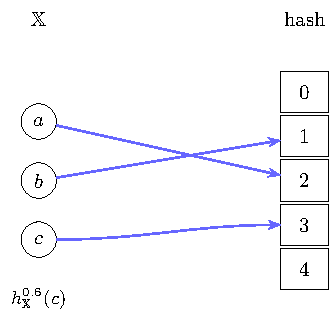
\includegraphics{pf}
\end{figure}

Every hash function in $\mathbbm{X} \mapsto \mathbbm{Y}$ is a perfect hash function over some subset of $\mathbbm{X}$, e.g., every hash function is trivially a perfect hash function of $\emptyset$ and singleton sets.

Assuming $\mathbbm{X}$ and $\mathbbm{Y}$ are finite, the set of hash functions of type $\mathbbm{X} \mapsto \mathbbm{Y}$, which may also be denoted by $\mathbbm{Y}^{\mathbbm{X}}$, has a cardinality
\begin{equation}
|\mathbbm{Y}|^{|\mathbbm{X}|}.
\end{equation}
The set of \emph{perfect} hash functions over $\mathbbm{A} \subseteq \mathbbm{X}$ is a subset of $\mathbbm{X} \mapsto \mathbbm{Y}$ with the predicate that no collisions may occur on any pair of elements in $\mathbbm{A}$.
The set of perfect hash functions over $\mathbbm{A}$ has a cardinality
\begin{equation}
\mathrm{permutations}(|\mathbbm{Y}|,|\mathbbm{A}|) |\mathbbm{Y}|^{|\mathbbm{X}| - |\mathbbm{A}|}.
\end{equation}

%####################################################################################################
% random oracle phf
%####################################################################################################

\section{A theoretical \emph{cryptographic} perfect hash function}
The bit set $\{0,1\}$ is denoted by $\{0,1\}$.
The set of all bit strings of length $n$ is therefore $\{0,1\}^n$.
The cardinality of $\{0,1\}^n$ is $2^n$.
In the case of $\{0,1\}$, we denote $\{0,1\}^0$ by $\epsilon$.
The set of all bit strings of length $n$ or less is denoted by $\{0,1\}^{\leq n}$ with a cardinality $2^{n+1}-1$, e.g., $\{0,1\}^{\leq 2} = \epsilon \cup \{0,1\} \cup \{0,1\}^2$.
The countably infinite set of all bit strings, $\lim_{n \to \infty} \{0,1\}^{\leq n}$, is denoted by $\{0,1\}^{*}$.
A tuple $(x_1,x_2\ldots) \in \{0,1\}^{*}$ is denoted a \emph{bit string}, and we typically drop the angle brackets when specifying strings, e.g., $(x_1,x_2) \equiv x_1 x_2$.

An important operation that is closed over the free semigroup of $\{0,1\}$ is \emph{concatentation}, $\cat : \{0,1\}^* \times \{0,1\}^* \mapsto \{0,1\}^*$, which is defined as $a_1 \ldots a_n \cat b_1 \ldots b_m = a_1 \ldots a_n b_1 \ldots b_m$ with special cases $x \cat \epsilon = \epsilon \cat x = x$.

Most hash functions are of the type $\{0,1\}^* \mapsto \{0,1\}^n$ where $n$ is some finite natural number.

Another useful function is the binary \emph{padding} function
$\mathrm{pad} : \{0,1\}^* \times \mathbbm{Z}_{\geq 0} \mapsto \{0,1\}^*$ is defined as $\mathrm{pad}(x,k) = x \cat 0^{k-\mathrm{BL}(x)}$ with the special case $\mathrm{pad}(x,0) = \epsilon$.


The binary \emph{truncation} function $\mathrm{trunc} : \{0,1\}^* \times \mathbbm{N} \mapsto \{0,1\}^*$ is defined as $\mathrm{trunc}(a_1 \ldots a_k \ldots a_n, k) = a_1 \ldots a_k$, with the special case $\mathrm{trunc}(x,0) = \epsilon$.

The \emph{bit length} function $\mathrm{BL} : \{0,1\}^* \mapsto \mathbbm{N}$ is defined as $\BL(a_1 \ldots a_n) = n$, e.g., if $b \in \{0,1\}^{n}$ then $\mathrm{BL}(b) = n$.

Since $\{0,1\}^* \cong \mathbbm{N}$, they may put into one-to-one correspondence.
A convenient one-to-one correspondence between them is given by the following definition.
\begin{definition}
	\label{def:mapping}
	The sets $\{0,1\}^*$ and $\mathbbm{N}$ have a bijection given by
	\begin{equation}
	b_1,\ldots,b_m \longleftrightarrow 2^m + \sum_{j=1}^{m} 2^{m - j} b_j.
	\end{equation}
\end{definition}

We denote the mapping described by Definition~\ref{def:mapping} with the postfix function $' : \{0,1\}^* \mapsto \mathbbm{N}$ and $' : \mathbbm{N} \mapsto \{0,1\}^*$, which are inverse functions, i.e., $x'' = x$.
An important observation of this mapping is that a natural number $n$ maps to a bit string $n'$ of length $\BL(n') = \lfloor \log_2 n \rfloor$.

More generally, if we have some set $\mathbbm{U}$, in a physical computer there must be a way to map the elements of $\mathbbm{U}$ to bit strings that \emph{represent} the values.
We provide this mapping with \emph{encoder} and \emph{decoder} functions denoted respectively by $\Fun{e}[\mathbbm{U}] : \mathbbm{U} \mapsto \{0,1\}^*$ and $\Fun{d}[\mathbbm{U}] : \{0,1\}^* \mapsto \mathbbm{U}$ such that $\Fun{d}[\mathbbm{U}] \circ e_\mathbbm{U} = \mathrm{id}_\mathbbm{U}$ and $e_\mathbbm{U} \circ d_\mathbbm{U} = \mathrm{id}_{\{0,1\}^*}$.

A special case of the encoder and decoder is given by letting any bit string represent either the sequence of bits $a_1 \ldots a_n$ or as the binary coded decimal (BCD), e.g., $010 \longleftrightarrow 4$.
Thus, any operation on non-negative integers may be applied to bit strings without ambiguity, e.g., $010 + 01 = 11$.

Given a function of $g : \mathbbm{X} \mapsto \mathbbm{Y}$, the \emph{domain} of $g$ may be denoted by $\mathrm{dom}(g) = \mathbbm{X}$ and the \emph{codomain} may be denoted by $\mathrm{codom}(g) = \mathbbm{Y}$.

A random oracle as given by the following definition.
\begin{definition}
\label{def:randomoracle}
A random oracle in the family $\{0,1\}^{*} \mapsto \{0,1\}^{\infty}$ is a theoretical \emph{hash function} whose output is uniformly distributed over its codomain.
\end{definition}

The theoretical analysis of the perfect hash function makes the following assumption.
\begin{assumption}
\label{asm:ro_approx}
The hash function $\mathrm{hash} : \{0,1\}^{*} \mapsto \{0,1\}^{\infty}$ is a random oracle.
\end{assumption}

%\begin{assumption}
%\label{asm:random_sets}
%The set $\mathbbm{S}$ consists of $m$ elements, where each element is drawn uniformly at random without replacement from $\{0,1\}^{*}$.
%\end{assumption}


\begin{definition}
The \emph{data type} for the \emph{cryptographic} perfect hash function under consideration is defined as $\PH = \{0,1\}^* \times \mathbbm{N}$ with a value constructor $\ph : \PS{\mathbbm{U}} \times [0,1] \mapsto \PH$ defined as
\begin{equation}
	\mathrm{ph}(\mathbbm{X}, r) = (n',N)
\end{equation}
where
\begin{equation}
\begin{split}
m			&= |\mathbbm{X}|,\\
N 			&= \lceil m / r \rceil,\\
k			&= \lceil\log_2 N\rceil,\\
\beta(x,n) 	&= \mathrm{trunc}\!\left(\mathrm{hash}(x' \cat n'),k\right)' \mod N,\\
\mathbbm{Y}_n 	&= \{\beta(x,n) \in \{0,\ldots,N-1\}|x \in \mathbbm{X}\},\\
n 			& = \min\{ j \in \mathbbm{N} | \mathbbm{Y}_j \in 2^{\mathbbm{N}} \land |\mathbbm{Y}_j| = m\}.
\end{split}
\end{equation}
\end{definition}

%A family of important functions of the form $\mathbbm{A} \times \mathbbm{B} \mapsto \mathbbm{A}$ and $\mathbbm{A} \times %\mathbbm{B} \mapsto \mathbbm{B}$ are respectively defined as $\Fun{fst}(\Tuple{a,b}) = a$ and %$\Fun{snd}(\Tuple{a,b}) = b$.

Since $\PH$ is a data type that purports to model perfect hash functions, its \emph{computational basis} is given by the following set of functions.

By the assumption of surjectivity (and the perfect hash function is not rated-distorted), then the load factor is given by $\frac{|\mathbbm{X}|}{N}$ where $N = \argmax_{x \in \mathbbm{X}} \mathrm{hash}_{\mathbbm{A}}(x)$, i.e., the maximum hash (natural ordering of integers) of $\mathrm{hash}_{\mathbbm{A}}$.
\begin{definition}
The \emph{minimum} and \emph{maximum} hash of a value of type $\PH$ (that models a perfect hash function) are given respectively by $\MinHash : \PH \mapsto \mathbbm{N}$ and $\MaxHash : \PH \mapsto \mathbbm{N}$ where
\begin{equation}
	\mathrm{min\_hash}(b,N) = 0\;\text{and}\;\mathrm{max\_hash}(b,N) = N-1.
\end{equation}
\end{definition}
%\begin{equation}
%	\MaxHash(t) = \Fun{snd}(t)-1.
%\end{equation}



The most important function, the \emph{perfect hash} mapping, $\mathrm{perfect\_hash} : \mathrm{PH} \times \mathbbm{U} \mapsto \mathbbm{N}$, is defined as
\begin{equation}
	\mathrm{ph}((b,N),x) = q' \mod N
\end{equation}
where
\begin{equation}
\begin{split}
	k &= \lceil \log_2 N \rceil,\\
	r &= \mathrm{hash}(x' \cat b),\\
	q &= \mathrm{trunc}(r,k).
\end{split}
\end{equation}



\begin{theorem}
	% dependent-type since codomain depends on r.
A value of type $\mathrm{PH}$ constructed with $\mathrm{ph}_{\{0,1\}^*}(\mathbbm{A},r)$ \emph{models} $\mathrm{hash}_{\mathbbm{A}}^{r} : \{0,1\}^* \mapsto \{0,1,\ldots,k-1\}$ where $\mathbbm{A} \subseteq \{0,1\}^*$ and $k = \frac{|\mathbbm{A}|}{r}$.
\end{theorem}
\begin{proof}
Let $(n', N) = \mathrm{ph}(\mathbbm{A}, r)$ be the value constructed by the definition. By construction, $N = \lceil |\mathbbm{A}|/r \rceil$, so the codomain has size $N = \lceil |\mathbbm{A}|/r \rceil \geq |\mathbbm{A}|/r$, yielding a load factor of at most $r$.

The value $n$ is chosen as the minimum natural number such that $|\mathbbm{Y}_n| = |\mathbbm{A}|$, where $\mathbbm{Y}_n = \{\beta(x,n) : x \in \mathbbm{A}\}$ and $\beta(x,n) = \mathrm{trunc}(\mathrm{hash}(x' \cat n'), k)' \mod N$. The condition $|\mathbbm{Y}_n| = |\mathbbm{A}|$ ensures that all elements of $\mathbbm{A}$ map to distinct hashes, i.e., $\beta(\cdot, n)|_{\mathbbm{A}}$ is injective.

The lookup function $\mathrm{perfect\_hash}((n', N), x)$ computes $\mathrm{trunc}(\mathrm{hash}(x' \cat n'), k)' \mod N$, which equals $\beta(x, n)$ by definition. Since $\beta(\cdot, n)|_{\mathbbm{A}}$ is injective and maps into $\{0, \ldots, N-1\}$, the function $\mathrm{perfect\_hash}((n', N), \cdot)$ restricted to $\mathbbm{A}$ is a perfect hash function with codomain $\{0, \ldots, N-1\}$ and load factor $|\mathbbm{A}|/N \leq r$.
\end{proof}

Suppose we have a function $f : \mathbbm{U} \mapsto \{0,1\}^*$ such that $f|_{\mathbbm{A}}$ is \emph{injective}, e.g., an \emph{encoder} for values of $\mathbbm{A} \subseteq \mathbbm{U}$.
The composition $\mathrm{hash}_{\mathbbm{A}} = \mathrm{hash}_{\mathbbm{B}} \circ f$ where $\mathbbm{B} = \{f(a) \in \{0,1\}^*|a \in \mathbbm{A}\}$ is a perfect hash function of type $\mathbbm{U} \mapsto \mathbbm{N}$ over $\mathbbm{A} \subseteq \mathbbm{U}$.
Thus, the rest of the material in this paper does not usually assume any particular domain of the perfect hash function since injections may always be constructed for any set.

\subsection{Analysis}
Note that since $n'$ denotes the geometric code for $n$ and we choose the smallest $n$ that succeeds, where each choice of $n$ is a geometrically distributed trial with probability $p$, the expected space complexity obtains the information-theoretic lower-bound of $1.44$ bits per element.


We search \emph{all} possible hash functions which are a function of $\mathrm{hash}$, an approximate random oracle, and choose the \emph{perfect hash function} on a specified set that has the \emph{smallest} bit length. We describe the algorithm for performing this exhaustive search in Algorithm~\ref{alg:ph}.


We consider a family of perfect hash functions for a set $\mathbbm{S}$ which are given by the output of a hash function $\mathrm{hash}$ that approximates a \emph{random oracle} applied to the input $x \in \mathbbm{S}$ concatenated with a bit string $b$. We describe the generative algorithm for the perfect hash function in Algorithm~\ref{alg:ph}. Note that in Algorithm~\ref{alg:ph}, the concatenation of two bit strings $x$ and $y$ is denoted by $x \cat y$.

The perfect hash function generated by Algorithm~\ref{alg:ph} has the statistical property that the output is uniformly distributed as given by the following theorem.
\begin{theorem}
The perfect hash function $\mathrm{hash}[\mathbbm{A}][r] : \mathbbm{X} \mapsto \{0,1,\ldots,k-1\}$, where $k = \frac{|\mathbbm{A}|}{r}$, is a random oracle over $\mathbbm{X} - \mathbbm{A}$ and the restriction $\mathrm{hash}_\mathbbm{A}^r| _{\mathbbm{A}} : \mathbbm{A} \mapsto \{0,1,\ldots,k-1\}$ is a random $k$-permutation oracle of $\mathbbm{A}$.
\end{theorem}
\begin{proof}
First, in Algorithm~\ref{alg:ph} on Line~5, $b_n$ is a bit string such that each $x \in \mathbbm{S}$ concatenated with $b_n$ hashes to a unique integer in $\{1,\ldots,N\}$ by the hash function $\mathrm{hash}$, thus the hash function found perfectly hashes the elements of $\mathbbm{S}$. 

Second, by Definition~\ref{def:randomoracle}, $\mathrm{hash}$ approximates a random oracle whose output is uniformly distributed over the elements of $\{0,1\}^{n}$. Viewing the elements of $\{0,1\}^{n}$ as integers, where $|\{0,1\}^n| = 2^n$, $\mathrm{hash}$ is uniformly distributed over $\{0,1,\ldots,2^n-1\}$.

If $N = k 2^n$ for some integer $k$, the remainder of the output of $\mathrm{hash}$ when dividing by $N$, given by the modulo operator, and adding $1$ is uniformly distributed over $\{1,\ldots,N\}$ since each $j \in \{1,\ldots,N\}$ has an equal number of hashes assigned to it by $\mathrm{hash}$. If $2^n \gg N$ and $N \neq k 2^n$ for some integer $k$, then it is approximately uniformly distributed and converges to the uniform distribution as $n \to \infty$.
\end{proof}

The probability that no collisions occur for a particular bit string in Algorithm~\ref{alg:ph} is given by the following theorem.
\begin{theorem}
The probability that a bit string $b \in \{0,1\}^{*}$ results in a perfect hash function is given by
\begin{equation}
\label{eq:p_m_N}
	p(m,r) = N^{-m} P^{N}_{m}
%    p(m,N) = \frac{N!}{N^m (N-m)!},
\end{equation}
where $m$ is the cardinality of the set being perfectly hashed, $r$ is the load factor, and $N = \frac{m}{r}$.
\end{theorem}
\begin{proof}
Suppose we have a set $\mathbbm{A} \subset \{0,1\}^*$ of cardinality $m$.
The set of perfect hash functions $\mathrm{hash}_{\mathbbm{A}}^{r} : \{0,1\}^* \mapsto \{0,1,\ldots,N-1\}$ restricted to $\mathbbm{A}$ where $N = \frac{m}{r}$ has a cardinality given by $P^{N}_{m}$ since any choice of $m$ out of $N$ elements in the codomain and any ordering of the $m$ elements in $\mathbbm{A}$ to the chosen $m$ elements in $\{0,1,\ldots,N-1\}$ satisfy the definition of perfect hashing.

%First, we must choose $m$ out of the $N$ elements in the codomain to perfectly hash the $m$ elements in $\mathbbm{A}$.
%There are a total of $N \choose m$ ways of doing this.
%Once we have chosen the $m$ elements, we do not care about the order in which we assign the $m$ elements in $\mathbbm{A}$ %to the $m$ elements in the codomain.
%There are a total of $m!$ such orderings, any of which satisfy the perfect hashing criteria.
%Thus, by the product rule, there are ${N \choose m} m! = P_{m}^{N}$ ways to make these choices.

The set of hash functions $\{0,1\}^* \mapsto \{0,1,\ldots,N-1\}$ restricted to $\mathbbm{A}$ has a cardinality of $N^m$.
Therefore, the ratio of perfect hash functions restricted to $\mathbbm{A}$ to the total hash functions restricted to $\mathbbm{A}$ is just
\begin{equation}
	p = \frac{P^{N}_{m}}{N^m}.
\end{equation}

By the property of the hash function $\mathrm{hash}^*$ being a random oracle, the algorithm randomly samples one of the hash functions, which is a perfect hash function with probability $p$.

%$\mathrm{hash}_{\mathbbm{A}}^{r}$ to $\mathbbm{A}$, there are $N^m$ hash functions of this type. type $\{0,1\}^* \mapsto \mathbbm{N}$ over $\mathbbm{A}$ with a load factor $r$ restricted to $\mathbbm{A}$ with 
	
%Suppose we have a set $\mathbbm{S} = \{x_1,\ldots,x_m\}$. First, we consider a singular set consisting of $x_1$. The probability that no collision occurs is $1$ since there are no other members to collide with. Second, we add $x_2$ to the set. The probability that no collision occurs is given by the probability
%\begin{equation}
%    \Prob{\mathrm{hash}(x_2 \cat b) \neq \mathrm{hash}(x_1 \cat b)} = \frac{N-1}{N}.
%\end{equation}
%This probability follows from the fact that out of the $N$ hashes to choose from, $N-1$ result in no collision. %Extending this logic, the probability that no collision occurs for all $m$ elements is given by
%\begin{align}
%    p(m,N)
%        &= \prod_{i=0}^{m-1} \frac{N - i}{N}\\
%        &= \frac{N!}{N^m (N-m)!}.
%\end{align}
\end{proof}

Equation (\ref{eq:p_m_N}) may be reparameterized with respect to the load factor. By (\ref{eq:loadfactor}), $r = m/N$. Solving this equation with respect to $N$ yields the solution
\begin{equation}
    N = \frac{m}{r},
\end{equation}
and thus plugging in this value of $N$ yields the result
\begin{equation}
\label{eq:p_m_r}
    p(m,r) = \frac{\left(\frac{m}{r}\right)!}{\left(\frac{m}{r}\right)^m \left(\frac{m}{r}-m\right)!}.
\end{equation}

The expected \emph{in-place} coding size is given by the following theorem.
\begin{theorem}
The expected coding size is given approximately by
\begin{equation}
\label{eq:code_size}
    \log_2 \mathrm{e} - \left(\frac{1}{r} - 1\right) \log_2\!\left(\frac{1}{1-r}\right) \text{ bits/element}.
\end{equation}
\end{theorem}
\begin{proof}
The space required for the perfect hash function found by Algorithm~\ref{alg:ph} is of the order of the length $n$ of the bit string $b_n$ in the returned tuple. Therefore, for space efficiency, the algorithm exhaustively searches for a bit string in the order of increasing size $n$.

We are interested in the first case when no collision occurs, which is a geometric distribution with probability of success $p(m,r)$ as given by the discrete random variable
\begin{equation}
    Q \sim \geodist\!\bigl(p\!\left(m,r\right)\bigr),
\end{equation}
where $p(m,r)$ is given by (\ref{eq:p_m_r}). The expected number of trials for the geometric distribution is given by
\begin{equation}
    \Expect{Q} = \frac{1}{p(m,r)} = \frac{\left(\frac{m}{r}\right)^m \left(\frac{m}{r}-m\right)!}{\left(\frac{m}{r}\right)!}.
\end{equation}
By Definition~\ref{def:mapping}, the $n$-th trial uniquely maps to a bit string of length $m = \lfloor \log_2 n \rfloor$. Thus, the expected bit length is given approximately by
\begin{align}
    \Expect{\log_2 Q}
        &= \log_2\!\left(\frac{\left(\frac{m}{r}\right)^m \left(\frac{m}{r}-m\right)!}{\left(\frac{m}{r}\right)!}\right)\\
        &= m \log_2\!\left(\frac{m}{r}\right) +
            \log_2\!\left(\frac{m}{r}-m\right)! - \log_2\!\left(\frac{m}{r}\right)! \; \text{ bits}.
\end{align}
By Stirling's approximation, 
\begin{equation}
    \log_2 n! \approx n \left(\log_2 n - \log_2 \mathrm{e}\right).
\end{equation}
and so the expectation may be rewritten approximately as
\begin{equation}
\begin{split}
    \Expect{Q} \approx &\;
        m \log_2\!\left(\frac{m}{r}\right) -
            \frac{m}{r} \left(\log_2\!\left(\frac{m}{r}\right) - \log_2 \mathrm{e}\right) +\\
        &\qquad\left(\frac{m}{r}-m\right) \left(\log_2\!\left(\frac{m}{r}-m\right) - \log_2 \mathrm{e} \right) \; \text{ bits}.
\end{split}
\end{equation}
Since we are interested in the expected \emph{bits per element}, we divide the expectation by $m$ and after further simplification arrive at
\begin{equation}
\begin{split}
    &\log_2\!\left(\frac{m}{r}\right) - \frac{1}{r} \log_2\!\left(\frac{m}{r}\right) +\\
    &\qquad \left(\frac{1}{r}-1\right) \log_2\!\left(\frac{m}{r}-m\right) + \log_2 \mathrm{e} \; \text{ bits/element}.
\end{split}
\end{equation}
After further simplification, we arrive at
\begin{equation}
    \log_2 \mathrm{e} - \left(\frac{1}{r} - 1\right) \log_2\!\left(\frac{1}{1-r}\right) \text{ bits/element}.
\end{equation}
\end{proof}

The encoding of the perfect hash function achieves maximum entropy for its expected length. Since $Q$ follows a geometric distribution with success probability $p = p(m,r)$, its entropy is given by
\begin{equation}
    H(Q) = \frac{-(1-p)}{p} \log_2(1 - p) - \log_2(p),
\end{equation}
which can be rewritten as
\begin{equation}
    H(Q) = \left(\frac{1}{p}-1\right) \log_2\!\left(\frac{1}{1 - p}\right) + \log_2\frac{1}{p}.
\end{equation}
This entropy equals the expected bit length $\mathbb{E}[\log_2 Q]$ derived above, confirming that the geometric coding of trial indices is entropy-optimal. The \emph{in-place} encoding---using the trial index $n$ directly as the stored bit string---achieves this maximum entropy because each bit string of length $\ell$ occurs with probability proportional to $q^{2^\ell - 1}(1 - q^{2^\ell})$, which matches the probability mass function of the random bit length $N$ derived in the Appendix.

\begin{theorem}[Maximum entropy encoding]
\label{thm:maxentropy}
The in-place encoding of the cryptographic perfect hash function achieves maximum entropy for its expected length. Specifically, for a perfect hash function over a set of cardinality $m$ with load factor $r$, the encoding $n'$ has entropy
\begin{equation}
H(N) = \mathbb{E}[\mathrm{BL}(n')] = \log_2 \mathrm{e} - \left(\frac{1}{r} - 1\right) \log_2\!\left(\frac{1}{1-r}\right) \text{ bits/element},
\end{equation}
which equals the information-theoretic lower bound for representing perfect hash functions over uniformly distributed random sets.
\end{theorem}
\begin{proof}
By the random oracle assumption, each trial $n$ succeeds independently with probability $p = p(m,r)$. The first successful trial $Q$ follows a geometric distribution, and the encoding $n'$ uses $\mathrm{BL}(n') = \lfloor \log_2 n \rfloor$ bits.

The entropy of a geometric random variable with success probability $p$ is $H(Q) = \frac{-(1-p)}{p}\log_2(1-p) - \log_2 p$. Since the bijection between $n$ and $n'$ preserves information, and the expected bit length equals the entropy, the encoding is optimal in the sense of Shannon's source coding theorem~\cite{shannon,coverandthomas}. No encoding can achieve a smaller expected length while faithfully representing the perfect hash function.
\end{proof}

Note that Algorithm~\ref{alg:ph} has an exponential time 
complexity with respect to the cardinality of the input set $\mathbbm{S}$. As a 
result, Algorithm~\ref{alg:ph} is not a practical algorithm for any reasonably large 
$m$. However, it is intended to illustrate theoretical properties useful to 
data structures that implement \emph{oblivious} sets and maps\cite{phf,pmf} 
based on the perfect hash function. Simple and efficient algorithms exist 
\cite{chd,simple}. 

The theoretical lower-bound of a \emph{minimal} perfect hash function is given by the following postulate.
\begin{postulate}
\label{pst:lb}
The theoretical lower-bound for \emph{minimal} perfect hash functions has an expected coding size given approximately by
\begin{equation}
\label{eq:low_bound}
    1.44\text{ bits/element}.
\end{equation}
\end{postulate}

\begin{theorem}
The cryptographic perfect hash generator given by Algorithm~\ref{alg:ph} results in a \emph{minimal} perfect hash function that obtains the theoretical lower-bound of $1.44\text{ bits/element}$ by invoking \makehash{$\cdot$, $r=1$}.
\end{theorem}
\begin{proof}
By (\ref{eq:code_size}), letting $r \to 1^{+}$ for the \emph{minimal} perfect hash results in an expected coding size given by
\begin{equation}
    \log_2 \mathrm{e} - \lim_{a \to 0^{-}} a \log_2 \frac{1}{a} = 1.44 \; \text{ bits/element},
\end{equation}
which is the expected lower-bound given by Postulate~\ref{pst:lb}.
\end{proof}
This is as expected, since Algorithm~\ref{alg:ph} finds the \emph{smallest} perfect hash function that is a function of a random oracle for any load factor $0 < r \leq 1$ in which the distribution of the sets are uniformly distributed. The following corollary follows as a result.
\begin{corollary}
The lower-bound for perfect hash functions with a load factor $0 < r \leq 1$ is given by (\ref{eq:code_size}).
\end{corollary}
As $r$ goes to $0$, the expected bits per element goes to $0$.

Note that the \emph{probability mass function} of the random bit string found for $b$ is known exactly. Thus, if the desire is to \emph{serialize} the perfect hash function for transmission or storage, shorter bit strings may be assigned to more probable bit strings. This representation is not usable \emph{in-place}, i.e., the serialization must be decoded, but it can reduce transmission or storage cost.

\begin{algorithm}
	\caption{Cryptographic perfect hash function constructor (single-level)}
	\label{alg:ph}
	\SetKwProg{func}{function}{}{}
	\KwIn
	{
		$\mathbbm{X} \subseteq \{0,1\}^*$ is the set to be perfectly hashed, and
		$r \in (0,1]$ is the load factor.
	}
	\KwOut
	{
		A perfect hash function of $\mathbbm{X}$ with load factor $r$, represented as $(b_n, N)$ where $N = \lceil |\mathbbm{X}|/r \rceil$.
	}
	\func{\makehash{$\mathbbm{X}$, $r$}}
	{
		$m \gets |\mathbbm{X}|$\;
		$N \gets \lceil m / r \rceil$\;
		$k \gets \lceil\log_2 N\rceil$\;
		\For{$n \gets 1$ \KwTo $\infty$}
		{
			$\mathbbm{Y} \gets \emptyset$\;
			$\alpha \gets \True$\;
			\For{$x \in \mathbbm{X}$}
			{
				$h \gets \mathrm{trunc}\!\left(\mathrm{hash}(x' \cat n'),k\right)' \mod N$\;
				\If{$h \in \mathbbm{Y}$}
				{
					$\alpha \gets \False$\;
					\Break\;
				}
				$\mathbbm{Y} \gets \mathbbm{Y} \cup \{h\}$\;
			}
			\If{$\alpha$}
			{
				\Return $(n', N)$\;
			}
		}
	}
\end{algorithm}

%############################################################################################################
% perf_hash_2_lvl_fn
%############################################################################################################
\section{A practical two-level perfect hash function}

\iffalse
\begin{algorithm}
	\caption{Two-level perfect hash function constructor}
	\label{alg:2ph_commented}
	\SetKwProg{func}{function}{}{}
	\KwIn
	{
		$\mathbbm{X} \subseteq \mathbbm{U}$ is the objective set,
		$r \in \{q \in \mathbbm{Q} | q \in 2^{-j} \land j \in \mathbbm{N}\}$ is a load factor, and
		$k \in \mathbbm{N}$ is the number of entries in the intermediate hash level.
	}
	\KwOut
	{
		A two-level perfect hash function of $\mathbbm{X} \subseteq \mathbbm{U}$ with a load factor $r$ and an intermediate level of $k$ indices, denoted by $\mathrm{hash}_{\mathbbm{X}}^{r} : \mathbbm{U} \mapsto \left\{0,\ldots,N\right\}$ where $N = \frac{|\mathbbm{X}|}{r}$.
	}
	\func{\mathrm{make\_hash}($\mathbbm{X}$, $r$, $k$)}
	{
		$t = \lceil \log_2 k \rceil$\;
		$N = \frac{|\mathbbm{X}|}{r}$\;
		\tcp{$\mathbbm{X}[0],\ldots,\mathbbm{X}[k-1]$ is a total partition of $\mathbbm{X}$.}
		$\mathbbm{X}[\ell] = \{x \in \mathbbm{X}|\mathrm{trunc}\!\left(\mathrm{hash}(x' \cat 0'),t\right)' \mod k = \ell}$\;
		$\mathbbm{Y} \gets \emptyset$\;
		\For{$\ell \in \{0,\ldots,k-1\}$}
		{
			\For{$n \gets 1$ \KwTo $\infty$}
			{
				$\mathbbm{Y}_\ell \gets \emptyset$\;
				$\alpha \gets \True$\;
				\For{$x \in \mathbbm{X}[\ell]$}
				{
					$\beta = \mathrm{trunc}\!\left(\mathrm{hash}(x' \cat n'),N\right)$\;
					\If{$\beta \in \mathbbm{Y}_\ell \cup \mathbbm{Y}$}
					{
						$\alpha \gets \False$\;
					}
					$\mathbbm{Y}_\ell \gets \mathbbm{Y}_\ell \cup \{\beta\}$\;
				}
				\If{$\alpha$}        
				{
					$\mathbbm{Y} \gets \mathbbm{Y} \cup \mathbbm{Y}_\ell$\;
					\Break\;
				}
			}
			%$A_\ell \gets n'$\;
			$\mathbbm{A} \gets \mathbbm{A} \cup \{(\ell,n)\}$\;
		}
		\tcp{A space-optimal serialization of $(\mathbbm{A},k,N)$ is $(\ln 2)^{-1}$ bits per element if $r$ is $1$.}
		\Return $(\mathbbm{A},k,N)'$
	}
\end{algorithm}
\fi


\begin{algorithm}
	\caption{Two-level perfect hash function constructor}
	\label{alg:2ph}
	\SetKwProg{func}{function}{}{}
	\KwIn
	{
		$\mathbbm{X} \subseteq \mathbbm{U}$ is the objective set, $r \in \{q \in \mathbbm{Q} | q \in 2^{-j} \land j \in \mathbbm{N}\}$ is the load factor, and $k \in \mathbbm{N}$ is the number of entries in the intermediate hash level.
	}
	\KwOut
	{
		A two-level perfect hash function of $\mathbbm{X} \subseteq \mathbbm{U}$ with a load factor $r$ and an intermediate level of $k$ indices, denoted by $\mathrm{hash}_{\mathbbm{X}}^{r} : \mathbbm{U} \mapsto \left\{0,\ldots,N\right\}$ where $N = \frac{|\mathbbm{X}|}{r}$.
	}
	\func{\makehash{$\mathbbm{X}$, $r$, $k$}}
	{
		$N = \frac{|\mathbbm{X}|}{r}$\;
		$t = \lceil \log_2 k \rceil$\;
		\tcp{$\mathbbm{X}[1],\ldots,\mathbbm{X}[k]$ is a total partition of $\mathbbm{X}$ and $\mathbbm{X}[j_1],\ldots,\mathbbm{X}[j_k]$ is in decreasing order of cardinality.}	
		$\mathbbm{X}[\ell] = \{x \in \mathbbm{X} \mid \mathrm{trunc}\!\left(\mathrm{hash}(x' \cat 0'),t\right)' \mod k = \ell\}$\;
		$\mathbbm{Y} \gets \emptyset$\;
		$\mathbbm{A} \gets \emptyset$\;		
		\For{$\ell \gets 1$ \KwTo $k$}
		{
			\For{$n \gets 1$ \KwTo $\infty$}
			{
				$\beta(x) = \mathrm{trunc}\!\left(\mathrm{hash}(x' \cat n'),N\right)$\;
				$\mathbbm{Y}_\ell = \{\beta(x) | x \in \mathbbm{X}[\ell]\}$\;
				\If{$|\mathbbm{Y}_\ell| = |\mathbbm{X}_\ell | \land \mathbbm{Y}_\ell \cap \mathbbm{Y} = \emptyset$}
				{
					$\mathbbm{Y} \gets \mathbbm{Y} \cup \mathbbm{Y}_\ell$\;
					\Break\;
				}
			}
			$\mathbbm{A} \gets \mathbbm{A} \cup \{(\ell,n)\}$\;
		}
		\Return $(\mathbbm{A},k,N)$
	}
\end{algorithm}

\subsection{Analysis}
Suppose we have a set $\mathbbm{X}$ of $m$ elements with some total order $x_{(1)},\ldots,x_{(m)}$ for which we seek a perfect hash function $\mathrm{hash}_{\mathbbm{X}} : \mathbbm{U} \mapsto \mathbbm{Z}$.

We denote the \emph{serialization} of some value $x$ by $x'$.
If $x$ is already understood to be a serialization, then $x'$ denotes deserialization instead.

By the assumption that the hash function $\mathrm{hash} : \mathbbm{U} \mapsto \{0,1\}^k$ is a random oracle restricted to the codomain $\{0,1\}^k$, the $n$-th attempt (trial) $\mathrm{hash}\!\left(x_{(j)}' \cat n'\right)$ to find a non-colliding hash for $x_{(j)}$ has a probability of success $p_j = \frac{m-j+1}{m}$ since we have already found hashes for the previous $j-1$ elements and therefore there are only $m-(j-1)$ hashes remaining.

This is an example of the Coupon collector's problem.
Let $T_j$ denote the uncertain number of trials needed to find a non-colliding hash for $x_{(j)}$.
The total number of trials needed is an uncertain random variable given by
\begin{equation}
T = \sum_{j=1}^{m} T_j.
\end{equation}
By the linearity of the expectation operator,
\begin{equation}
E(T) = \sum_{j=1}^{m} E(T_j) = \sum_{j=1}^{m} \frac{1}{p_j} = m H_{m-1},
\end{equation}
which asymptotically converges to $E(T) = m \gamma + m \ln(m-1)$ or on average $\gamma + \ln (m-1)$ trials per element of $\mathbbm{X}$.

If we use the minimum number of bits to encode each trial index $n$ for each bucket, the expected space per bucket is $\log_2 \mathrm{e} \approx 1.44$ bits, matching the single-level lower bound. However, the two-level approach offers a practical advantage: by partitioning the set into $k$ smaller buckets, each bucket requires fewer trials on average, reducing construction time from exponential in $m$ to polynomial.

The variance of $T$ is given by
\begin{equation}
\mathrm{Var}(T) = \sum_{j=2}^{m} \mathrm{Var}(T_j).
\end{equation}
Since each $T_j$ follows a geometric distribution with success probability $p_j = \frac{m-j+1}{m}$, we have $\mathrm{Var}(T_j) = \frac{1-p_j}{p_j^2}$, and thus
\begin{equation}
\mathrm{Var}(T) = \sum_{j=2}^{m} \frac{j-1}{(m-j+1)^2} \cdot m^2.
\end{equation}
This variance is $O(m^2)$, indicating that while the expected number of trials grows as $m \ln m$, the actual number of trials can vary significantly for any particular set.

The two-level construction in Algorithm~\ref{alg:2ph} trades space optimality for construction efficiency. By processing buckets in decreasing order of cardinality, larger buckets are assigned hashes first when more slots are available, reducing the expected number of collisions with previously assigned hashes.

%############################################################################################################
% composition
%############################################################################################################

\section{Algebra of function composition}

Perfect hash functions can be composed with other functions to create new perfect hash functions with different properties. This algebraic structure provides flexibility in designing hash function families.

\subsection{Composition preserves injectivity}

While a perfect hash function $h_\mathbbm{A} : \mathbbm{X} \mapsto \mathbbm{Y}$ is not globally injective, its restriction to $\mathbbm{A}$ is injective:
\begin{equation}
	h_\mathbbm{A}|_{\mathbbm{A}} : \mathbbm{A} \mapsto \mathbbm{Y}.
\end{equation}
This restriction property enables composition with injective functions while preserving the perfect hash property.

\begin{theorem}[Post-composition with injection]
Let $g : \mathbbm{Y} \mapsto \mathbbm{Z}$ be an injective function, $h_\mathbbm{A}^r : \mathbbm{X} \mapsto \mathbbm{Y}$ be a perfect hash function, and $|\mathbbm{Z}| = (1 + \alpha) |\mathbbm{Y}|$ for $\alpha \geq 0$.
The composition $g \circ h_\mathbbm{A}^r : \mathbbm{X} \mapsto \mathbbm{Z}$ is a perfect hash function $h_\mathbbm{A}^{r'}$ where $r' = \frac{r}{1+\alpha}$.
\end{theorem}
\begin{proof}
From the load factor definition, $r = \frac{|\mathbbm{A}|}{|\mathbbm{Y}|}$, so $|\mathbbm{Y}| = \frac{|\mathbbm{A}|}{r}$.
Since $g$ is injective, $g \circ h_\mathbbm{A}^r$ is injective on $\mathbbm{A}$, making it a perfect hash function with load factor
\begin{equation}
	r' = \frac{|\mathbbm{A}|}{|\mathbbm{Z}|} = \frac{|\mathbbm{A}|}{(1+\alpha)|\mathbbm{Y}|} = \frac{|\mathbbm{A}|}{(1+\alpha)\frac{|\mathbbm{A}|}{r}} = \frac{r}{1+\alpha}.
\end{equation}
\end{proof}

\subsection{Permutation equivalence classes}

Given a perfect hash function $h_\mathbbm{A} : \mathbbm{X} \mapsto \mathbbm{Y}$, composing with any permutation $\pi : \mathbbm{Y} \mapsto \mathbbm{Y}$ yields another perfect hash function $\pi \circ h_\mathbbm{A}$ over $\mathbbm{A}$ with the same load factor. Since there are $|\mathbbm{Y}|!$ permutations of $\mathbbm{Y}$, a single perfect hash function generates a family of $|\mathbbm{Y}|!$ related perfect hash functions.

These functions form an \emph{equivalence class} where all members have identical collision structure outside of $\mathbbm{A}$. This equivalence class can be denoted $[\pi \circ h_\mathbbm{A}]$ where $\pi$ ranges over all permutations of $\mathbbm{Y}$.

\begin{corollary}
For a perfect hash function with codomain $\mathbbm{Y}$, the ratio of permutation-equivalent perfect hash functions to all possible functions is
\begin{equation}
	\frac{|\mathbbm{Y}|!}{|\mathbbm{Y}|^{|\mathbbm{X}|}}.
\end{equation}
\end{corollary}

\subsection{Applications of composition}

The algebraic properties of perfect hash function composition have practical applications in several contexts.

\begin{example}
\textbf{Domain adaptation.} Suppose we have a perfect hash function $h_\mathbbm{A} : \{0,1\}^* \mapsto \{0,\ldots,N-1\}$ constructed by Algorithm~\ref{alg:ph}, but we require a hash function over a different domain $\mathbbm{U}$. Given any injective encoder $e : \mathbbm{U} \mapsto \{0,1\}^*$, the composition $h_\mathbbm{A} \circ e$ is a perfect hash function over $e^{-1}(\mathbbm{A}) \subseteq \mathbbm{U}$ with the same load factor.
\end{example}

\begin{example}
\textbf{Load factor adjustment.} Given a minimal perfect hash function ($r = 1$), we can reduce the load factor to any $r' < 1$ by composing with an injection $g : \{0,\ldots,N-1\} \hookrightarrow \{0,\ldots,\lceil N/r' \rceil - 1\}$. This allows trading space for reduced collision probability outside of $\mathbbm{A}$.
\end{example}

\begin{example}
\textbf{Randomization.} Given a deterministic perfect hash function, composing with a random permutation $\pi$ yields a randomized perfect hash function that preserves the perfect hash property while obscuring the original hash assignments. This is useful in cryptographic applications where predictability of hash values is undesirable.
\end{example}

These composition properties demonstrate that perfect hash functions form a rich algebraic structure, enabling flexible construction of hash function families from primitive building blocks.

%############################################################################################################
% appendix
%############################################################################################################

\appendix
\appendixpage
\addappheadtotoc
\section{Probability mass of random bit length}
\begin{algorithm}
    \caption{Bit length sampler of the cryptographic perfect hash function}
    \label{alg:sampler}
    \SetKwProg{func}{function}{}{}
    \KwIn
    {
        The number $m$ is the cardinality of the perfect hash set and
        the number $r$ is the load factor.
    }
    \KwOut
    {
        The \emph{minimum bit length} $n$ conditioned on a random set of cardinality $m$ and a load factor $r$.
    }
    \func{$\sampler(m, r)$}
    {
        \For{$i \gets 1$ \KwTo $m$}
        {
            $x \gets \text{randomly draw a bit string from $\{0,1\}^{*}$ without replacement}$\;
            $\mathbbm{S} \gets \mathbbm{S} \cup \{x\}$\;
        }    
        $(b_n,N) \gets \makehash\left(\mathbbm{S}, r\right)$\;
        \tcp{The integer $N$ must also be coded, which we assume has a constant bit length.}
        \Return $n + \mathcal{O}(1)$\;
    }
\end{algorithm}
The bit length of the perfect hash function found by Algorithm~\ref{alg:ph} has an uncertain value with respect to (random) sets and therefore we may model it as a random variable as given by the following definition.
\begin{definition}
\label{def:N_rv}
The perfect hash function generated by Algorithm~\ref{alg:ph} has a random bit length given by
\begin{equation}
    N = \sampler(m,r)
\end{equation}
where $m$ is the cardinality of the random set and $r$ is the load factor.
\end{definition}
Note that if the distribution of sets is not uniformly distributed as given by 
\sampler, then better algorithms than Algorithm~\ref{alg:ph} are possible, i.e., the 
lower-bounds are with respect to \emph{uniformly distributed}
random sets and smaller lower-bounds are possible if the random sets are 
non-uniformly distributed.

The probability mass of the random bit length $N$ is given by the following theorem.
\begin{theorem}
\label{thm:N_pmf}
The random bit length $N$ has a probability mass function given by
\begin{equation}
\label{eq:N_pmf}
    p_N(n | m, r) = q^{2^n-1}\left(1 - q^{2^n}\right).
\end{equation}
where $m$ is the cardinality of the random set, $r$ is the load factor, and $q = 1 - p(m,r)$, 
\end{theorem}
\begin{proof}
Each iteration of the loop in Algorithm~\ref{alg:ph} has a collision test which is Bernoulli distributed with a probability of success $p(m,r)$, where success denotes no collision occurred. We are interested in the random length $N$ of the bit string when this outcome occurs.

For the random variable $N$ to realize a value $n$, every bit string smaller than length $n$ must fail and a bit string of length $n$ must succeed. There are $2^n-1$ bit strings smaller than length $n$ and each one fails with probability $q$, and so by the product rule the probability that they all fail is given by
\begin{equation}
\label{eq:N_pmf_1}
    q^{2^n - 1}.
\end{equation}

Given that every bit string smaller than length $n$ fails, what is the probability that every bit string of length $n$ fails? There are $2^n$ bit strings of length $n$, each of which fails with probability $q$ as before and thus by the product rule the probability that they all fail is $q^{2^n}$, whose complement, the probability that not all bit strings of length $n$ fail, is given by
\begin{equation}
\label{eq:N_pmf_2}
    1 - q^{2^n}.
\end{equation}
By the product rule, the probability that every bit string smaller than length $n$ fails and a bit string of length $n$ succeeds is given by the product of (\ref{eq:N_pmf_1}) and (\ref{eq:N_pmf_2}),
\begin{equation}
\label{eq:prob_is_mass}
    q^{2^n-1}\left(1 - q^{2^n}\right).
\end{equation}
For (\ref{eq:prob_is_mass}) to be a probability mass function, two conditions must be met. First, its range must be a subset of $[0,1]$. Second, the summation over its domain must be $1$.

The first case is trivially shown by the observation that $q$ is a positive number between $0$ and $1$ and therefore any non-negative power of $q$ is positive number between $0$ and $1$.

The second case is shown by calculating the infinite series
\begin{align}
    S &= \sum_{n=0}^{\infty} q^{2^n-1}\left(1-q^{2^n}\right)\\
      &= \sum_{n=0}^{\infty} q^{2^n-1} - q^{2^{n+1}-1}.
\end{align}
Explicitly evaluating this series for the first $4$ terms reveals a telescoping sum given by
\begin{equation}
    S = (1 - q) + (q - q^3) + (q^3 - q^7) + (q^7 - q^{15}) + \cdots,
\end{equation}
where everything cancels except $1$.
\end{proof}

In Figure~\ref{fig:pmf_fN}, we plot the probability mass function of $N$ conditioned on $m=25$ and several different load factors. We see that the probability mass is peaked and unimodal and tends to nearly zero everywhere except over a concentrated interval around its expected value.
\begin{figure}
\centering
\caption{Probability mass function of\\random bit length $N$}
\label{fig:pmf_fN}
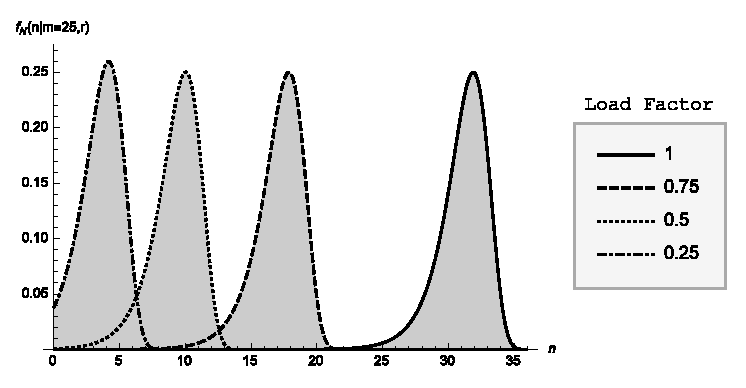
\includegraphics{plotfn}
\end{figure}

The expected size was already computed, but the probability mass function contains everything there is to know about the distribution of $N$, not just the \emph{expected} value. However, for illustration, we show how the expected value may be computed.
\begin{theorem}
\label{thm:open_expect}
The expected bit length of $N$ conditioned on random sets of cardinality $m$ and a load factor $r$ is given by
\begin{equation}
\label{eq:alt_expectN}
    \Expect{N} = \sum_{j=1}^{\infty} q^{2^j-1},
\end{equation}
where $q = 1 - p(m,r)$.
\end{theorem}
\begin{proof}
The expectation of $N$ is given by
\begin{align}
    &\sum_{j=0}^{\infty} j q^{2^j-1}\left(1 - q^{2^j}\right)\\
    &\qquad=\sum_{j=0}^{\infty} j \left(q^{2^j-1} - q^{2^{j+1}-1}\right).
\end{align}
Explicitly evaluating this series for the first $4$ terms reveals a converging sum given by
\begin{align}
    &0 + (q - q^3) + 2(q^3 - q^7) + 3(q^7 - q^{15}) + \cdots\\
    &\qquad= q + q^3 + q^7 + q^{15} + \cdots.
\end{align}
\end{proof}
When we numerically evaluate (\ref{eq:alt_expectN}) for various $m$ and $r$, the results are in agreement with (\ref{eq:code_size}).


%\listoffigures
%\listofalgorithms

\bibliographystyle{plain}
\bibliography{references}
\end{document}

